%%%%%%%%%%%%%%%%%%%%%%%%%%%%%%%%%%%%%%%%%
% Beamer Presentation
% LaTeX Template
% Version 1.0 (10/11/12)
%
% This template has been downloaded from:
% http://www.LaTeXTemplates.com
%
% License:
% CC BY-NC-SA 3.0 (http://creativecommons.org/licenses/by-nc-sa/3.0/)
%
%%%%%%%%%%%%%%%%%%%%%%%%%%%%%%%%%%%%%%%%%

%----------------------------------------------------------------------------------------
%    PACKAGES AND THEMES
%----------------------------------------------------------------------------------------

\documentclass[aspectratio=169]{beamer}

\mode<presentation> {

\usetheme{CambridgeUS}

}

\usepackage{graphicx} % Allows including images
\usepackage{url}
\usepackage{hyperref}
\usepackage{amsthm}

\DeclareGraphicsExtensions{.png, .jpg, .pdf}

\setlength{\parskip}{1em}

%----------------------------------------------------------------------------------------
%    TITLE PAGE
%----------------------------------------------------------------------------------------

\title[The Travelling Salesman Problem]{Quantum Speedup of the Travelling Salesman Problem on Bounded Degree Graphs} % The short title appears at the bottom of every slide, the full title is only on the title page

\author[Dominic J. Moylett]{Dominic J. Moylett\footnote{Work completed in collaboration with Ashley Montanaro and Noah Linden.}} % Your name
\institute[University of Bristol] % Your institution as it will appear on the bottom of every slide, may be shorthand to save space
{
School of Physics and Department of Electrical and Electronic Engineering\\
University of Bristol \\ % Your institution for the title page
\medskip
\textit{\href{mailto:dominic.moylett@bristol.ac.uk}{dominic.moylett@bristol.ac.uk}} % Your email address
}
\date{\today} % Date, can be changed to a custom date

\begin{document}

\begin{frame}
\titlepage % Print the title page as the first slide
\end{frame}

%----------------------------------------------------------------------------------------
%    PRESENTATION SLIDES
%----------------------------------------------------------------------------------------

%------------------------------------------------
\section{Introduction}
%------------------------------------------------

\begin{frame}
\frametitle{Based on a True Story}
\begin{columns}[T]
\begin{column}{.5\textwidth}
I graduated in June 2015.

To celebrate, I wanted to do a tour of Europe.
\end{column}
\begin{column}{.5\textwidth}
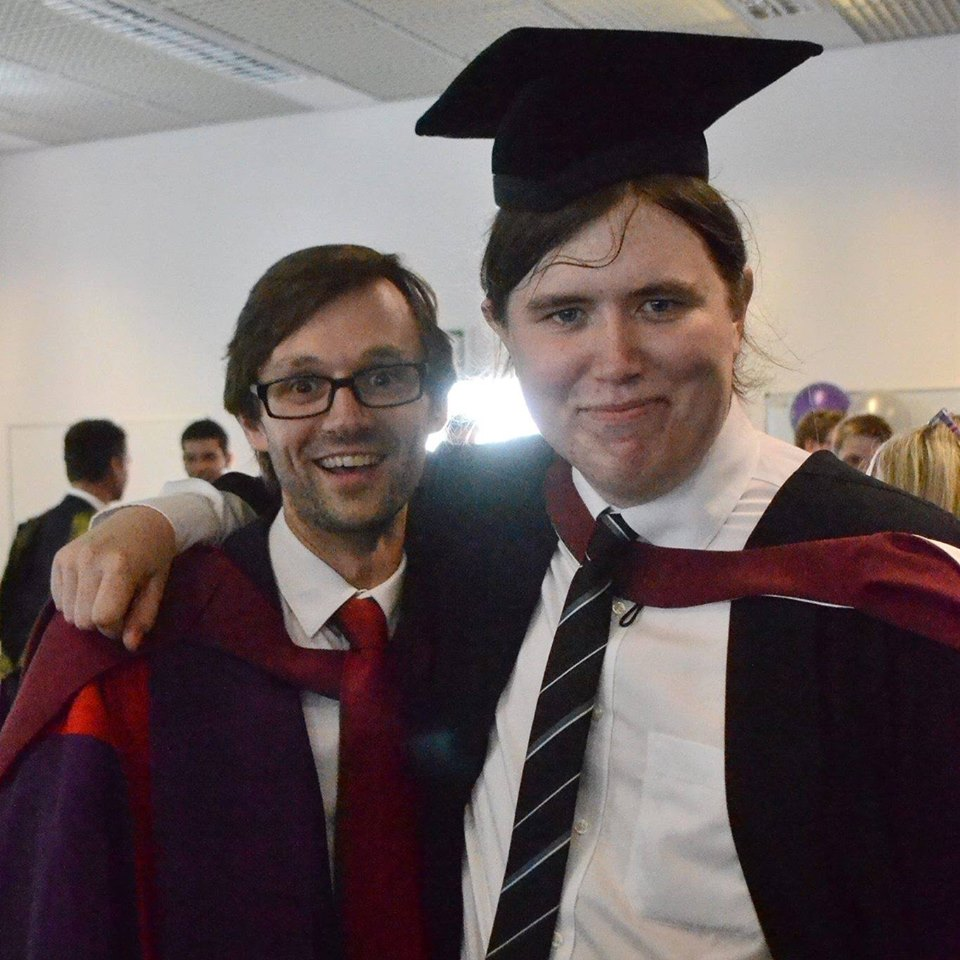
\includegraphics[scale=0.15]{graduation}
\end{column}
\end{columns}
\end{frame}

\begin{frame}
\frametitle{Interrail}
\begin{center}
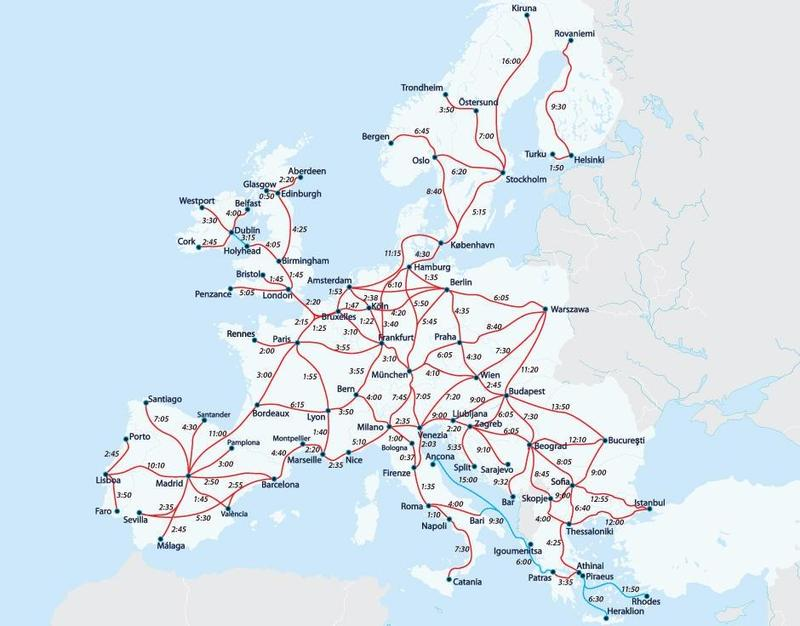
\includegraphics[scale=0.35]{interrail}\footnote{\url{http://www.interrail.eu/plan-your-trip/interrail-railway-map}}
\end{center}
\end{frame}

\begin{frame}
\frametitle{Where we wanted to visit}
\begin{center}
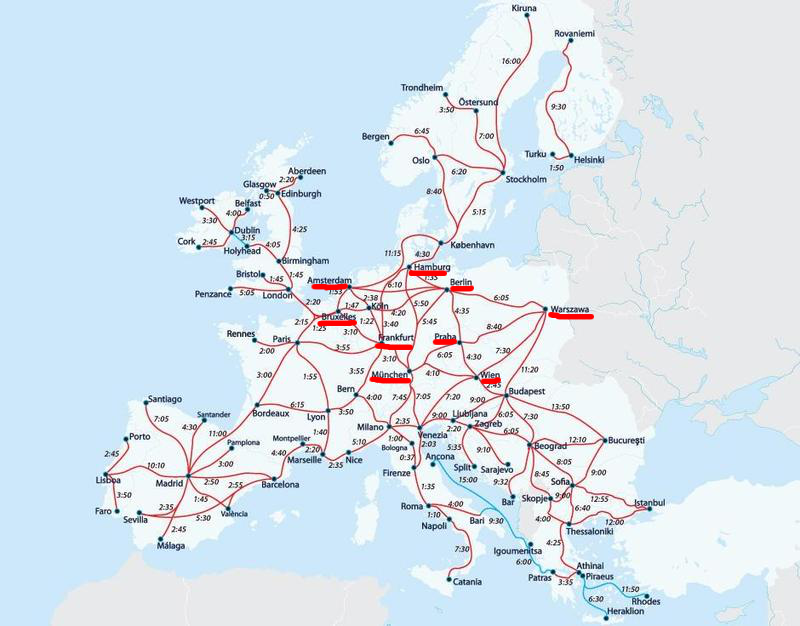
\includegraphics[scale=0.25]{interrail_selected}
\end{center}
What's the fastest way of visiting every location?
\end{frame}

\begin{frame}
\frametitle{The Travelling Salesman Problem}
\begin{columns}[T]
\begin{column}{.5\textwidth}
Given a graph $G = (V, E)$ with cost matrix $C$, what is Hamiltonian cycle with the lowest cost?

This problem is $NP$-hard, so finding a polynomial time solution would prove that $P = NP$.

A na\"ive solution would take $O(|V|!)$ time by searching over every permutation of the vertices.

Grover search could be applied to this approach to achieve $O(\sqrt{|V|!})$ time.

But other more efficient classical algorithms exist. Can these be sped up using quantum algorithms?
\end{column}
\begin{column}{.5\textwidth}
TODO: Add graph.
\end{column}
\end{columns}
\end{frame}

\begin{frame}
\frametitle{Our Results}
\begin{itemize}
\item A quadratic speedup for the Travelling Salesman Problem when the degree of any vertex in the graph is at most $3$.
\item This is using a classical algorithm by Eppstein\footnote{D.\ Eppstein, {\em Journal of Graph Algorithms and Applications}, {\bf 11}(1), pp.\ 61--81 (2007)}, combined with a quantum speedup by Montanaro\footnote{A.\ Montanaro, {\em arXiv:1509.02374}}.
\item Speedups for graphs of higher bounded degrees are found by reducing to this case.
\end{itemize}
\end{frame}

%------------------------------------------------
\section{How to not speed up the Travelling Salesman Problem}
%------------------------------------------------

\begin{frame}
\frametitle{The Difficulty of a Quantum Speedup}

Key components for many algorithms have limited interesting quantum speedup:

\begin{itemize}
\item The Held-Karp algorithm\footnote{M.\ Held and R.\ M.\ Karp, {\em Journal of the Society for Industrial and Applied Mathematics}, {\bf 10}(1), pp.\ 196-210 (1962)} relies on dynamic programming (no known speedup).
\item Christofides' algorithm\footnote{N.\ Christofides, {\em Management Sciences Research Report 388, Graduate School of Industrial Administration, CMU} (1976)} relies on finding a minimum weight perfect matching (speedup for bipartite graphs).
\item Algorithms which use Nearest Neighbour can be sped up from $O(n^2)$ to $O(n^{3/2})$ time via Grover search.
\end{itemize}

Others algorithms do not even have known performance\footnote{S. Kirkpatrick, C.\ D.\ Gelatt and M.\ P.\ Vecchi, {\em Science}, {\bf 220}(4598), pp.\ 671--680 (1983)}.
\end{frame}

%------------------------------------------------
\section{Travelling Salesman Problem on Cubic Graphs}
%------------------------------------------------

\begin{frame}
\frametitle{Eppstein's Algorithm}
Solves the Travelling Salesman Problem on graphs where the degree of any vertex is at most $3$.

Takes as input a graph $G = (V, E)$ and a set $F \subseteq E$ of ``forced'' edges.

Returns the shortest Hamiltonian cycle which includes every edge in $F$.

Main steps:
\begin{itemize}
\item Reduce $(G, F)$ to $(G', F')$ by changing specific subgraphs in $G$.
\item If $F'$ contains a Hamiltonian cycle then return then length of $F'$.
\item If a Hamiltonian cycle cannot be made, then abort.
\item Pick an edge $xy \in V' \setminus F'$ according to specific rules.
\item Call Eppstein's algorithm on $(G', F' \cup \{xy\})$ and $(G' \setminus \{xy\}, F')$.
\item Return the Hamiltonian cycle length with the shortest path. If both branches abort then abort.
\end{itemize}
\end{frame}

\begin{frame}
\frametitle{Edge Picking}
The main bottleneck of Eppstein's algorithm is the recursive calls. So how is the edge to force or remove chosen?

\begin{enumerate}
\item If $G' \setminus F'$ has a cycle of four vertices such that two of the vertices are incident to forced edges, pick one vertex $x$ in the cycle that is not incident to a forced edge and another vertex $y$ not in the cycle.
\item Otherwise if $F' \neq \emptyset$, pick an edge $(y, z) \in F$ and then chooses an adjacent edge $(x, y) \notin F$ as long as $(x, y)$ is not part of a disjoint cycle of four vertices in $G \setminus F$.
\item Otherwise pick any edge.
\end{enumerate}

\end{frame}

\begin{frame}
\frametitle{Performance}
Eppstein showed that these branching rules broke the problem size into one of two cases:

\begin{enumerate}
\item A subproblem with two more forced edges and one more cycle of $4$ unforced edges, and a subproblem with three fewer vertices.
\item Two subproblems with three more forced edges.
\item A subproblem with two more forced edges, and a subproblem with five more forced edges.
\end{enumerate}

Linear recurrence solving shows that the overall runtime of is $O(2^{n/3})$.
\end{frame}

\begin{frame}
\frametitle{Why not use Grover search?}
Grover search can be used if we can map a binary string to each result of the algorithm.

We can apply Grover search to Eppstein's algorithm by removing an edge if the next bit is $0$ and forcing it if the next bit is $1$.

However, the longest bit string we might need is $n/2$ bits, because of the case which only which only adds two forced edges to the graph.

Thus the best speedup we would see of Grover search is $O(2^{n/4})$ time.

We need to take advantage of the problem's structure if we want to do even better.
\end{frame}

\begin{frame}
\frametitle{Backtracking Algorithms}
Backtracking algorithms are algorithms to solve constraint satisfaction problems, where we have $n$ variables to assign values to such that they satisfy $m$ constraints.

They work by using a predicate $P$ and heuristic $h$ as follows, given a partial assigment $V$:

\begin{enumerate}
\item If $P(V) = \bot$ then abort.
\item Let $v_{i} \leftarrow h(V)$.
\item For all possible assignments $a$ to $v_{i}$:
\begin{enumerate}
\item Call recursively on $(V \cup (v_{i}, a))$
\item If call does not abort then return $(V \cup (v_{i}, a))$.
\end{enumerate}
\item Abort.
\end{enumerate}
\end{frame}

\begin{frame}
\frametitle{Quantum Speedup for Backtracking Algorithms}

Montanaro proved the following:

\begin{theorem}[Montanaro]
Let $T$ be the number of recursive calls made by a backtracking algorithm. For any $0 < \delta < 1$, there is a quantum algorithm which evaluates $P$ and $h$ $O(\sqrt{T}n^{3/2}\log(n)\log(1/\delta))$ times, and outputs a partial assignment $V$ such that $P(V)$ is true or aborts if no such $V$ exists. The algorithm fails with probability $\delta$.
\end{theorem}

This speedup works by visualising the backtracking algorithm's calls as a tree and performing a quantum walk on the tree.
\end{frame}

%------------------------------------------------
\section{Conclusion}
%------------------------------------------------

\begin{frame}
\frametitle{Conclusion}
Future Steps:
\begin{itemize}
\item Apply further analysis to algorithms by Xiao and Nagamochi to see if they can perform even better.
\item See if we can outperform Bjorklund et al.\ for bounded degree $7$.
\item ???
\item Publish!
\end{itemize}
\end{frame}

%------------------------------------------------
\section{The End}
%------------------------------------------------

\begin{frame}
\frametitle{The End}
\begin{center}
Any questions?

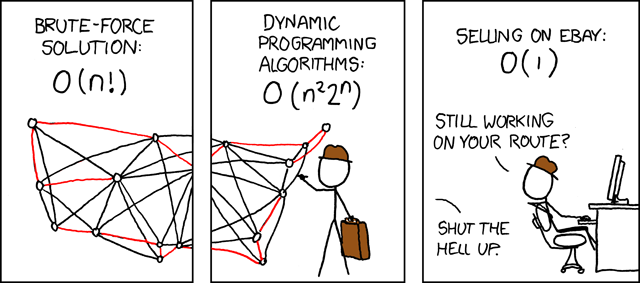
\includegraphics[scale=0.5]{xkcd}\footnote{\url{https://xkcd.com/399/}}
\end{center}
\end{frame}

%------------------------------------------------
\section{Post-credits}
%------------------------------------------------

\begin{frame}
\frametitle{Post-credits}
\centerline{This is not the slide you're looking for.}
\end{frame}

%----------------------------------------------------------------------------------------

\end{document} 
